\documentclass{article}
\usepackage{graphicx, soul, amsmath}
\usepackage[dvipsnames]{xcolor}
\usepackage[a4paper, margin=0.8in]{geometry}
\usepackage{fancyhdr} % Paquete para encabezados y pies de página

% Configuración de soul
\setul{0.5ex}{0.3ex}

% Comandos personalizados
\newcommand{\ulcolor}[2][Red]{\setulcolor{#1}\ul{#2}}
\newcommand*\sepline{%
  \begin{center}
    \rule[1ex]{.5\textwidth}{.5pt}
  \end{center}}

% Configuración de encabezado y pie de página para todas las páginas
\fancypagestyle{main}{
    \fancyhf{} % Limpia encabezados y pies de página
    \fancyhead[C]{Juan Ignacio Elosegui} % Encabezado centrado con tu nombre
    \fancyfoot[R]{\thepage} % Número de página alineado a la derecha en el pie
    \renewcommand{\headrulewidth}{0.4pt} % Línea bajo el encabezado
    \renewcommand{\footrulewidth}{0pt}   % Sin línea en el pie de página
}

% Aplicar el estilo por defecto a todo el documento
\pagestyle{main}

\title{Teoría de las Decisiones $-$ Comportamiento (Resumen)}
\date{Noviembre 2024}

\begin{document}

    % Primera página con título y encabezado
    \maketitle
    \thispagestyle{main} % Asegura el estilo en la primera página

    \section*{\underline{Módulo 1: Sesgos (Parte 1)}}
        \subsection*{Predictably Irrational - Ariely (Relativity)}
            \textbf{Ejemplo:} tenemos tres opciones para leer el diario \textit{The Economist}. Nos podemos suscribir al portal web por US\$59, podemos recibir una versión impresa por US\$125, pero también podemos estar suscritos y recibir una versión impresa por US\$125.
            \begin{center}
                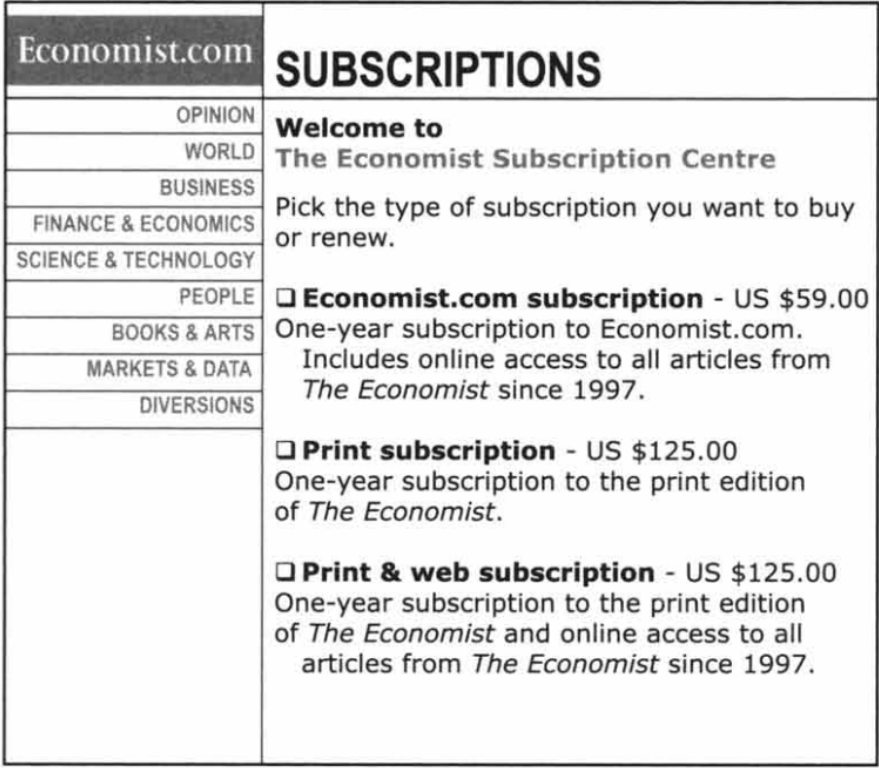
\includegraphics[width=0.5 \linewidth]{figs/sesgos.png}
            \end{center}
            ¿Quién querría comprar solamente la versión impresa, cuando podés conseguir la versión impresa y la suscripción a la página web por el mismo precio?

            Básicamente te están manipulando así terminás comprando la opción más cara de todas: versión impresa y la suscripción a la página web.

            Las personas en general no eligen las cosas en términos absolutos. No tenemos una forma de medir el valor de las cosas definida, si no que pensamos en las ventajas relativas de una cosa por sobre otra y su valor estimado. Esto pasa cuando pensamos que un auto de 8 cilindros debería ser más caro que un auto de 4 cilindros.
            \\
            \\
            En \textit{The Economist}, no tenía la menor idea de que la suscripción de US\$59 era "mejor" que la versión impresa de US\$125, pero claramente sabía que el combo suscripción y versión impresa por US\$125 es claramente mejor que menos cosas con el mismo precio.

            Esto quiere decir que la gente no sabe lo que quiere hasta que lo ve en algún contexto como este, el problema es que todo es relativo.
            \\
            \\
            Si no te diste cuenta, a la gente no le gusta pensar, parece ser muy complicado y poco placentero. Si existieran sólo dos opciones, US\$59 por la suscripción en la web y US\$125 por la versión impresa es una decisión un poco más complicada.

            Los clientes ven difícil computar el valor de las diferentes opciones. En este caso, la mayoría de las personas van a elegir la opción del medio.

            Por más que no querramos, siempre vemos las cosas en comparación a las otras. Sin importar la dificultad de la decisión. Comparamos las cosas fáciles, y no tenemos ganas de comparar las cosas difíciles.

    \sepline

    \section*{\underline{Módulo 2: Sesgos (Parte 2)}}
        \subsection*{Predictably Irrational - Ariely (Anchoring)}
            \textbf{Contexto:} la armada estadounidense necesitaba relojes a prueba de agua. James Assael, a través de sus contactos en Suiza, pudo suplir esta demanda.
            
            Cuando la guerra terminó, el contrato de Assael con el gobierno de Estados Unidos terminó y el tipo se quedó con miles de relojes suizos. Japón necesitaba relojes, claro, pero no tenían guita; lo único que tenían los japoneses eran perlas.

            El hijo de Assael había aprendido el oficio de comerciar relojes suizos por perlas japonesas. Su negocio prosperó, y se consagró como el "Rey de las Perlas".

            Como se hizo millonario, consiguió un atolón en Tahití que casualmente tenía perlas negras, pero estas perlas no valían nada porque no había mercado para eso. Esperó un año para que consiga mejores perlas y se las dió a un amigo para que las venda recontra caras en Nueva York.
            \\
            \\
            ¿Cómo convenció a la sociedad para que se vuelvan locos por estas perlas? Pasa algo parecido con las crías de los gansos: cuando nacen, se apegan psicológicamente a lo primero que ven (generalmente, su madre). A este fenómeno se le llama \emph{anclaje}. Lo que hizo Assael es esto: ancló sus perlas junto a las gemas más preciosas del mundo, y sus precios se acoplaron ahí para siempre.
            \\
            \\
            Básicamente, con el anclaje se prueba que la coherencia arbitraria es cuando se nos dan precios iniciales, estos son "arbitrarios". Cuando ya están marcados en nuestra cabeza. Entonces, nos anclamos a precios iniciales.

        \subsection*{Misbehaving, The Making of Behavioral Economics - Thaler (Fairness)}
            Imaginate que en Viedma hay una plaga de mosquitos nunca antes vista. No se puede salir a la calle de los mosquitos que hay, con dengue encima. Querés ir a La Anónima o a la farmacia a comprar Off y ves que está al doble de precio. ¿Cómo reaccionás? Esto es totalmente racional desde un punto de vista económico -porque se mantiene la oferta y aumenta considerablemente la demanda, entonces aumentará el precio- pero varias personas pueden considerar injusto eso.

            Esto se relaciona con el principio de doble titularidad: los consumidores sienten que tienen derecho a un precio de referencia, y las empresas tienen derecho a proteger sus beneficios (como aumentar el Off), pero no a explotar a sus consumidores.
            \\
            \\
            La equidad como la conocemos no siempre coincide con los modelos económicos tradicionales, pero es importante entender el comportamiento humano en la práctica.
            
    \sepline

    \section*{\underline{Módulo 3: Manejando la Incertidumbre}}
        \subsection*{Caso Carter}
            Trata de una escudería de carreras, que está analizando si presentarse a correr la última carrera de la temporada o no. Esta última carrera es muy importante no sólo por la plata que podrían ganar, si no por la exposición que tendría Carter Racing.
            
            Si les va medianamente bien conseguirían más sponsors, la posibilidad de ver ganancias y el lujo de competir con los equipos más importantes del mundo. Pero si llegaran a tener otra falla del motor en televisión nacional esto no sería bueno.
            \\
            \\
            El mecánico del equipo pensaba que los problemas del motor estaban relacionados con la baja temperatura ambiente. El día de la carrera amaneció con temperaturas bajo cero, por lo que, al momento de la carrera, seguramente haga frío.

            Analizando los pocos datos que tenían a disposición, se dieron cuenta que las fallas del motor se dan en distintas temperaturas: por lo que no necesariamente se rompe el motor cuando hace frío.

            La escudería tenía que sentarse a pensar en el día si iban a correr la carrera o no. Si corren y pierden otro motor, se funden ellos también. A los muchachos se les presentó una toma de decisiones bajo riesgo, porque 1) efectivamente están bajo riesgo, y 2) pueden saber con qué probabilidad va a fallar el motor.
            \\
            \\
            No hay mucho para analizar, sólo que es ejercicio práctico para analizar la toma de decisiones bajo incertidumbre y presión. Sin embargo, está inspirado en el desastre del transbordador espacial Challenger en 1986, y su desenlace se utiliza para reflexionar sobre cómo decisiones similares pueden conducir a consecuencias graves si no se consideran adecuadamente los riesgos.
        \subsection*{Expected Monetary Value Theory (EMVT)}
            Es una teoría prescriptiva que provee una receta para elegir la opción que, en promedio, genera la mayor ganancia. Fue la herramienta que usaron los de Carter Racing para saber si correr o no la carrera \ldots
            \\
            \\
            Consideremos una aseguradora que tiene que decidir si asegurar o no a un individuo. El seguro cuesta \$100 por el próximo año (no hay obligación de renovarlo) y, en caso de muerte, la aseguradora debe pagar \$25.100. Luego de realizarle estudios médicos al individuo, la aseguradora estimó que existe una probabilidad del 5\% de que esa persona muera en el próximo año. ¿Debe o no debe asegurarlo?
            \\
            \begin{table}[h]
                \begin{tabular}{ccc}
                                & Muere & Vive \\
                    Asegurar    & \ulcolor[Red]{$- \mathdollar 25.000$}, \ulcolor[Green]{$0,05$} & \ulcolor[Red]{$+ \mathdollar 100$}, \ulcolor[Green]{0,95} \\
                    No asegurar & \ulcolor[Red]{$\mathdollar 0$}, \ulcolor[Green]{0,05} & \ulcolor[Red]{$\mathdollar 0$}, \ulcolor[Green]{0,95} \\
                \end{tabular}
            \end{table}
            Calculamos el EMV de cada opción.
            \\
            \(EMV_{Asegurar} = -\mathdollar 25.000 \cdot 0,05 + \mathdollar 100 \cdot 0,95\) \\
            \(EMV_{Asegurar} = -\mathdollar 1.155\) \\ \\
            \(EMV_{No asegurar} = \mathdollar 0 \cdot 0,05 + \mathdollar 0 \cdot 0,95\) \\
            \(EMV_{No asegurar} = \mathdollar 0\) \\
            \\
            Esta empresa no va a asegurar al individuo, porque se espera que pierdan más plata si lo aseguran.

            Acá la empresa de seguros está haciendo una decisión bajo riesgo, porque no saben si se va a morir el cliente o no, pero conocen la probabilidad de que eso pase. Entonces, lo que hicieron fue calcular el EMV, donde intervienen los pagos posibles y las probabilidades. Las cuentas son fáciles de sacar, no jodan.

            Se le dice "riesgo" ni bien intervienen las probabilidades, porque se la están jugando. La decisión es si lo aseguran o no, y es el puntapié de un árbol de decisiones. Si aseguran a la persona, están asumiendo el riesgo de que muera o que no muera el próximo año, no se sabe qué va a pasar.
            \\
            \\
            El \textit{Expected Value given Perfect Information (EV|PI)} -o, para los hinchas de Boca, el Valor Esperado dada Información Perfecta- representa el resultado monetario máximo que obtendríamos si tuviéramos la certeza absoluta sobre cuál será el resultado de un evento. Es decir, si conociéramos con anticipación cuál de todas las posibles opciones se va a dar.
            \\
            El \textit{Expected Value of Perfect Information (EVPI)} se calcula restando el EMV al EV$|$PI. Esta diferencia nos indica cuánto mejoraría nuestra situación si pudiéramos eliminar la incertidumbre y tomar siempre la decisión correcta, en comparación con tomar la decisión basada en las probabilidades actuales. En otras palabras, es cuánto estaríamos dispuestos a pagar a cambio de recibir información perfecta.
            \\
            \\
            Supongamos que un inversor está decidiendo si invertir en acciones, bonos o un plazo fijo. El retorno las primeras dos inversiones depende de si la economía crece, se mantiene o decrece en el próximo año. Si la economía crece (y lo hará con 50\% de probabilidad), las acciones darán un retorno de \$1500 y los bonos \$900. Si la economía se mantiene (30\% de probabilidad), las acciones darán \$300 y los bonos \$600. Si la economía decrece (20\% de probabilidad), se perderán \$800 en el caso de las acciones y \$200 en el caso de los bonos. El plazo fijo, en cambio, da un retorno de \$500 sin importar lo que ocurra con la economía.
            \\
            \begin{table}[h]
                \begin{tabular}{cccc}
                                & Crece         & Mantiene      & Decrece       \\
                    Acciones    & \ulcolor[Red]{$+1.500$}, 0,5 & $+300$, 0,3   & $-800$, 0,2   \\
                    Bonos       & $+900$, 0,5   & \ulcolor[Red]{$+600$}, 0,3   & $-200$, 0,2   \\
                    Plazo Fijo  & $+500$, 0,5   & $+500$, 0,3   & \ulcolor[Red]{$+500$}, 0,2   \\
                \end{tabular}
            \end{table}
            Calculamos el EMV de cada opción.
            \\
            \(EMV_{Acciones} = 1.500 \cdot 0,5 + 300 \cdot 0,3 + (-800) \cdot 0,2 \) \\
            \(EMV_{Acciones} = 680 \) \\ \\
            \(EMV_{Bonos} = 900 \cdot 0,5 + 600 \cdot 0,3 + (-200) \cdot 0,2 \) \\
            \(EMV_{Bonos} = 590 \)\\ \\
            \(EMV_{Plazo Fijo} = 500 \cdot 0,5 + 500 \cdot 0,3 + 500 \cdot 0,2\) \\
            \(EMV_{Plazo Fijo} = 500\)\\ \\
            Puede parecer una pelotudez lo que estoy por decir -algo que no es novedad-, pero poner los símbolos de $\mathdollar$ es totalmente innecesario. Entre más, mejor.
            
            Como las acciones le dan un EMV mayor que cualquier otra cosa, será donde invierta el inversor.
            \\
            \\
            ¿Cuánto pagaría para eliminar el riesgo?
            \\
            \(EV|PI = (EV|Crece) \cdot P(Crece) + (EV|Mantiene) \cdot P(Mantiene) + (EV|Decrece) \cdot P(Decrece)\) \\
            \textit{Sabemos que si la economía crece, le hubiera gustado haber invertido en acciones ($1.500 > 900 > 500$); si se mantiene le hubiera gustado haber invertido en bonos ($600 > 500 > 300$) y si decrece le hubiera gustado haber invertido en plazo fijo ($500 > -200 > -800$). El inversor ve lo que más rédito le da viendo las columnas.} \\
            \(EV|PI = 1.500 \cdot 0,5 + 600 \cdot 0,3 + 500 \cdot 0,2\) \\
            \(EV|PI = 1.030\) \\
            \\
            \(EVPI = EV|PI - EMV_{Acciones}\) \\
            \textit{Usamos el EMV que le daba más plata al inversor, que era invertir en acciones. Más dudoso que un amigo de tu novia.}\\
            \(EVPI = 1.030 - 680\) \\
            \(EVPI = 350\)
    
    \sepline

    \section*{\underline{Módulo 4: Distorsionando la Incertidumbre}}
        \subsection*{La Ruleta Rusa - Riesgo Extremo}
            Supongamos que un enemigo nos obliga a jugar a la ruleta rusa, pero dado que tiene tantas ganas de vernos morir, nos insta a jugar a una versión muy particular. En esta versión, si tenemos la suerte de sobrevivir el primer disparo, vamos a girar aleatoriamente la cámara y volver a disparar. La única opción que nos da nuestro “benévolo” enemigo es elegir con qué pistola jugar dentro de las siguientes dos opciones: \\
            Opción A: Jugar con una pistola que tiene 2 balas en posiciones desconocidas. \\
            Opción B: Elegir al azar (con 50\% de probabilidad) entre dos pistolas, una que tiene 1 bala y otra que tiene 3 balas (también en posiciones desconocidas). \\
            \\
            Si calculáramos las chances de sobrevivir, nos daríamos cuenta de que existe en la opción A un 44\% de probabilidad de sobrevivir dos disparos, y que, en la opción B existe un 47\% de chance de sobrevivir dos disparos.

            Aunque el número medio de balas disparadas es el mismo, la opción B ofrece mayores probabilidades de supervivencia. Este análisis demuestra que pequeñas diferencias en las probabilidades pueden influir en las decisiones, aunque el valor esperado de balas disparadas sea igual.

            En las decisiones bajo riesgo no sólo intervienen los valores esperados, si no que también hay que evaluar las probabilidades.
        \subsection*{Paradoja de San Petersburgo}
            Esta paradoja la propuso un Bernoulli y la resolvió otro Bernoulli (\ldots). Se trata de una apuesta donde cada lanzamiento de una moneda balanceada duplica el premio, comenzando desde \$2. El EMV de esta apuesta es infinito, pero la mayoría de las personas no están dispuestas a pagar mucho por participar. ¿Por qué pasa esto? \\
            \\
            El Bernoulli que la resolvió dijo que existe una función de utilidad logarítmica, diciendo que las personas no maximizan los EMV, si no su \emph{utilidad esperada}. Básicamente, lo que quiere decir, es que la utilidad en cuanto a dinero es algo logarítmico (una función que crece rápido al principio y luego crece cada vez menos).

            Esto resuelve la paradoja al mostrar que el infinito de la serie no refleja cómo percibimos realmente los valores monetarios, porque a medida que aumenta la serie, nos genera una utilidad cada vez menor.
        \subsection*{Expected Utility Theory (EUT)}
            La teoría de utilidad esperada (EUT) la formalizaron John von Neumann y Oskar Morgenstern. Describe cómo los agentes racionales toman decisiones bajo incertidumbre buscando maximizar la \emph{utilidad esperada} en vez del valor monetario esperado. La gente racional suele tener tres comportamientos posibles frente al riesgo:
            \begin{itemize}
                \item Aversión al riesgo: la gente no se la quiere jugar. Quiere patear fuerte y al medio por más que el valor esperado sea el mismo.
                \item Simpatía por el riesgo: la gente prefiere jugársela si hay recompensas importantes.
                \item Neutralidad al riesgo: la gente es indiferente entre jugársela o no con el mismo valor esperado.
            \end{itemize}
            Si tenemos dos opciones: \\
            Opción A: 50\% de ganar \$1.000 y 50\% de no ganar nada. \\
            Opción B: Ganar \$500 seguro.\\
            \\
            Si fuéramos aversos al riesgo no nos la vamos a jugar. Eligiríamos B porque buscamos las opciones seguras. \\
            Si fuéramos simpáticos al riesgo nos la jugamos. Eligiríamos A porque hay una recompensa importante. \\
            \\
            Estos muchachos también creen que para que un agente sea considerado racional este debe usar reglas de probabilidad para decidir, debe preferir alternativas con mayor utilidad o probabilidad y debe tener preferencias transitivas y consistentes.
        \subsection*{Ley de Weber-Fechner - La Percepción Subjetiva}
            La percepción humana de estímulos (como el dinero) sigue una escala logarítmica, según esta ley.

            Quiere decir que si tenemos un estímulo cada vez más intenso, vamos a necesitar cambios de intensidad de estos estímulos también cada vez más grandes para que notemos una diferencia. Esto es como decir que ganar \$100 es bastante más impactante para mí que para una persona millonaria.

    \sepline
            
    \section*{\underline{Módulo 5: Rompiendo la Teoría}}
        \subsection*{Paradoja de Allais: La Inconsistencia de las Preferencias}
            Las elecciones humanas pueden ser inconsistentes con la EUT \ldots \\
            \\
            Veamos dos escenarios: \\
            \\
            Escenario 1: \\
            Opción A: \$1.000.000 con 100\% \\
            Opción B: \$1.000.000 con 89\%, \$5.000.000 con 10\% o \$0 con 1\% \\
            \\
            Escenario 2: \\
            Opción A: \$1.000.000 11\% o \$0 con 89\% \\
            Opción B: \$5.000.000 con 10\% o \$0 con 90\% \\
            \\
            Resulta que muchas personas eligen A en el escenario 1, y B en el escenario 2. Estas decisiones no respetan la regla de la independencia de las alternativas irrelevantes, que es un principio fundamental de la EUT. Si una opción es preferida a otra en una comparación directa, esa preferencia no debería cambiar al añadir una tercera opción irrelevante (es decir, que no afecta la comparación original).

            Lo que están haciendo la mayoría de las personas, deja en evidencia que, frente a algunos escenarios (y teniendo en cuenta el contexto) son aversas al riesgo (como asegurarse el millón en el Escenario 1) y, para otros escenarios, son simpatizantes al riesgo (porque no les importa tener un millón con mayor probabilidad, se la jugaron por los cinco millones en el Escenario 2).

            Si tenés una preferencia entre dos opciones en un contexto cualquiera, deberías mantenerla por más que el contexto cambie. \\
            \\
            El cambio de preferencia, para Allais, demuestra que los humanos no siempre somos coherentes. Esto sugiere que nuestras decisiones no se basan únicamente en cálculos racionales, sino también en factores psicológicos, como la aversión a la pérdida o la percepción del riesgo.
        \subsection*{Paradoja de Ellsberg: Aversión a la Ambigüedad}
            Esta paradoja, propuesta por Daniel Ellsberg, demuestra cómo las personas prefieren opciones con probabilidades conocidas sobre aquellas ambiguas, incluso cuando la EUT sugiere que deberían ser indiferentes. \\
            \\
            Veamos dos escenarios: una urna tiene 90 bolitas: 30 son rojas, 60 son amarillas o azules (no conocemos la proporción) \\
            \\
            Escenario 1: \\
            Opción A: \$100 si sale una bolita roja \\
            Opción B: \$100 si sale una bolita amarilla \\
            \\
            Escenario 2: \\
            Opción A: \$100 si sale una bolita amarilla o azul (\textit{¿quién es el bostero que hace las diapositivas?}) \\
            Opción B: \$100 si sale una bolita roja o azul \\
            \\
            Muchas personas eligieron A en el Escenario 1 porque prefieren conocer las probabilidades, en este caso la de sacar una bolita roja.
            
            Pero en el Escenario 2 las personas terminan contradiciéndose a ellos y al principio de las utilidades esperadas (se ignora que la opción A y B tienen exactamente la misma probabilidad). Esto evidencia una \emph{aversión a la ambigüedad}, porque la gente evita tomar decisiones si las probabilidades son inciertas. Se "vieron asustadas" por esta incertidumbre de proporción entre bolitas azules y amarillas. \\
            \\
            Por lo tanto, para Daniel Ellsberg, la gente no siempre calcula probabilidades o utilidades esperadas para tomar decisiones.

    \sepline

    \section*{\underline{Módulo 6: Una Teoría Irracional}}
        \subsection*{Prospect Theory}
            Kahneman y Tversky descubrieron que hay limitaciones en la EUT para explicar comportamientos que pasan en la práctica. Propusieron la \emph{Prospect Theory} (PT), que tiene tres fundamentos:
            \begin{itemize}
                \item Aversión a las pérdidas: el dolor de perder es más fuerte que el placer de ganar una cantidad equivalente.
                \item Las evaluaciones que la gente hace acerca de las ganancias o las pérdidas depende de un punto de referencia. No se toman las decisiones sólo en base al valor total que tenemos, si no con lo que esperábamos tener -o sea, de dónde partimos-.
                \item La gente sobreestima probabilidades pequeñas y subestiman las probabilidades altas.
            \end{itemize}
            Jack y Jill tienen hoy \$5.000.000. Pero ayer Jack tenía \$1.000.000 (tuvo una ganancia de cuatro millones) y Jill tenía \$9.000.000 (tuvo una pérdida de cuatro millones).

            Los dos tienen un punto de referencia distinto (que es la plata que tenían ayer), pero Jack será más feliz que Jill por la comparación de su billetera de un día al otro. \\
            \\
            Antonio tiene \$1.000.000, y tiene que tomar una decisión: \\
            Opción A: 50\% de seguir con un \$1.000.000 o 50\% de terminar con \$4.000.000 \\
            Opción B: terminar con \$2.500.000 seguro \\
            \\
            Antonio elige B porque valora más la certeza de ganar \$2.500.000 que la posibilidad de obtener más. \\
            \\
            Betty tiene \$4.000.000 y tiene que tomar una decisión: \\
            Opción A: 50\% de terminar con un \$1.000.000 o 50\% de seguir con \$4.000.000 \\
            Opción B: terminar con \$2.500.000 seguro \\
            \\
            Betty elige A prefiere arriesgarse para evitar la pérdida total, incluso si eso podría resultar en un peor resultado. \\
            \\
            En el contexto de ganancias, Antonio prefiere asegurar un resultado positivo menor en lugar de arriesgarse por uno mayor. Esto es típico de una \emph{aversión al riesgo}, común cuando las personas se sienten cómodas con la certeza de un resultado seguro.

            Al comparar \$2.5 millones con la posibilidad de mantener \$4 millones o caer a \$1 millón, Betty toma decisiones basadas en evitar pérdidas significativas (en su marco mental). En el dominio de las pérdidas, las personas suelen mostrar \emph{simpatía por el riesgo}, aceptando más incertidumbre para evitar resultados dolorosos.
            \\
            \\
            La aversión al riesgo en ganancias se puede ver con el siguiente ejemplo: \\
            \\
            Opción A: ganar \$240 seguro \\
            Opción B: 25\% de ganar \$1.000 y 75\% de ganar nada \\
            \\
            La mayoría prefiere A, sólo porque es un resultado garantizado. No importa que la opción riesgosa B tenga un EMV más alto de \$240. El beneficio psicológico de la certeza pesa más que el EMV de la incertidumbre, por lo que patean fuerte y al medio \ldots \\
            \\
            La simpatía por el riesgo en pérdidas se puede ver con este ejemplo: \\
            Opción A: perder \$740 seguro \\
            Opción B: 75\% de perder \$1.000 y 25\% de no perder nada \\
            \\
            La mayoría prefiere B porque, cuando se trata de pérdidas, las personas son más propensas a asumir riesgos. Perder \$740 es tiene un impacto psicológico más negativo que la pérdida esperada de la incertidumbre de la opción B. Aunque la pérdida esperada es ligeramente mayor, la probabilidad de evitar completamente la pérdida (25\%) pesa más emocionalmente \ldots
        \subsection*{Aversión a las Pérdidas}
            Es un sesgo cognitivo que explica lo siguiente:
            \begin{itemize}
                \item Efecto dotación: las personas valoran más lo que ya tienen.
                \item Sesgo de status quo: la gente prefiere mantener el estado actual. "Si funciona, no lo cambies".
                \item Las ofertas como las "pruebas gratis" en alguna aplicación funcionan porque no nos gusta perder algo que supimos tener.
            \end{itemize}
        \subsection*{Distorsión de Probabilidades}
            La gente no procesa las probabilidades objetivamente, si no que juegan también los pesos psicológicos. \\
            \\
            Como dije antes, la gente sobreestima probabilidades pequeñas (efecto de posibilidad) y subestima las probabilidades altas (efecto de certeza).

            Si aumenta de 0\% a 5\% la probabilidad de un terremoto mañana en Viedma se va a generar un impacto más grande que si esa misma probabilidad pasa de 50\% a 55\%.
        \subsection*{Nueva Función de Utilidad}
            La función de Prospect Theory es asimétrica y depende de un punto de referencia llamado $R$: \\
            \[
                u(v, R) =
                \begin{cases} 
                  -(R - v)^{\beta} & \text{si } v < R \\ 
                  (v-R)^{\alpha} & \text{si } v \geq R.
                \end{cases}
            \]
            Con $\alpha < \beta < 1$, significa que hay una sensibilidad menos a las ganancias que a las pérdidas y existe un mayor impacto psicológico de las pérdidas. \\
            \\
            En la rama de las ganancias ($v \geq R$), hay un crecimiento cada vez menor y una aversión al riesgo en este dominio. \\
            En la rama de las pérdidas ($v < R$), es una función convexa, hay un mayor impacto psicológico y una simpatía por el riesgo en este dominio. \\

    \sepline

    \section*{\underline{Módulo 7: Una Teoría Alternativa \ldots}}
        \subsection*{El Juego}
            Supongamos que tenemos que lanzar una moneda al aire. Si sale cara (H), se gana el 50\% de la riqueza actual; si es ceca (T), se pierde el 40\%. \textit{Para los hinchas de Boca, se usa 'heads' para cara y 'tails' para ceca}.

            Si calculamos el valor esperado, nos va a parecer ventajoso jugar a este juego, porque si tenemos una riqueza inicial llamada $x$, tenemos un EMV que es $1,05 \cdot x$.\\
            Pero hay un problema: si el EMV es positivo, ¿por qué la mayoría de la gente termina con menos riqueza después de varias rondas?
        \subsection*{Ergocidad}
            Un proceso es \emph{ergódico} si los promedios temporal y ensamblado coinciden.

            Un promedio temporal es el crecimiento a lo largo del tiempo para un individuo, y un promedio ensamblado es un promedio entre múltiples universos posibles.

            Los procesos no ergódicos, como este juego, generan resultados diferentes. Además, el valor esperado sobreestima el resultado individual típico porque solo algunos jugadores se benefician, mientras la mayoría pierde riqueza.
        \subsection*{Economía de la Ergocidad}
            \begin{itemize}
                \item Crítica a la Teoría Tradicional: la teoría de utilidad tradicional asume que los individuos pueden aprovechar el promedio entre múltiples universos, algo que es imposible para las decisiones individuales.
                \item Por lo tanto, se busca evaluar el promedio temporal (tasa de crecimiento de riqueza a lo largo del tiempo) para que refleje mejor las consecuencias reales para una persona.
            \end{itemize}
            \begin{center}
                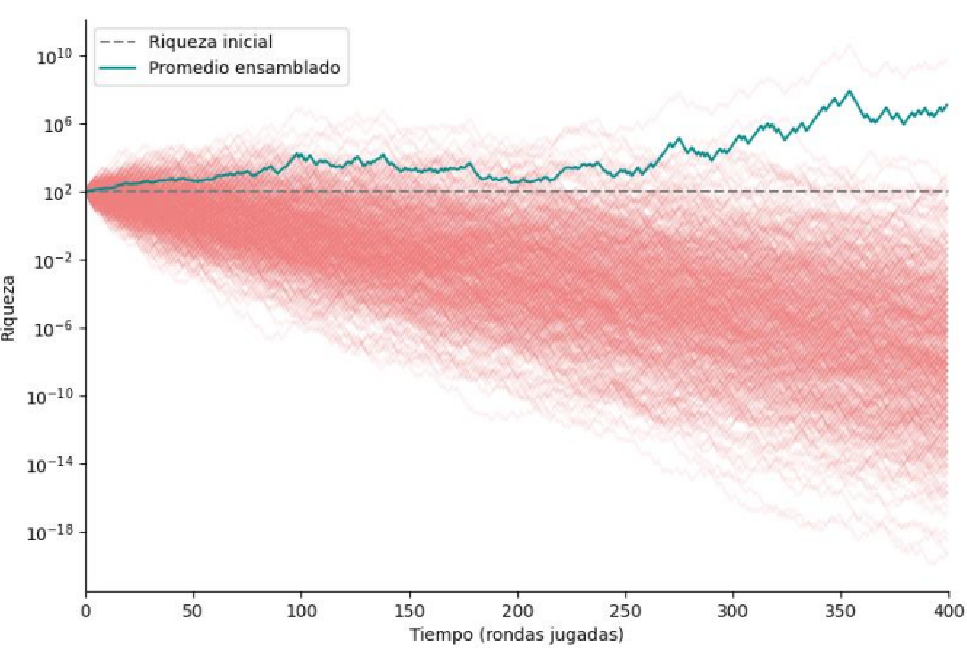
\includegraphics[width=0.85 \linewidth]{figs/ergocidad.PNG}
            \end{center}
             Incluso con 1000 jugadores y 400 rondas (para cada jugador), la riqueza promedio del grupo puede aumentar mientras la mayoría pierde riqueza.

             En cuanto al grupo, en cada ronda, se calcula el promedio de la riqueza de los jugadores. Este promedio, generalmente, muestra un crecimiento continuo. \\
             En cuanto a los individuos, la mayoría de estos jugadores pierde riqueza después de unas pocas rondas. Esto pasa porque la dinámica multiplicativa del juego no favorece a los jugadores de manera uniforme. La riqueza de unos pocos jugadores crece desproporcionadamente, elevando el promedio grupal, mientras que muchos otros terminan con menos de lo que tenían al principio.

             Aunque las simulaciones muestran un incremento en la riqueza promedio grupal, esto no refleja la realidad de la mayoría de los jugadores. El enfoque tradicional de basarse en el valor esperado (promedio ensamblado) es engañoso porque oculta los riesgos individuales asociados con procesos no ergódicos. \\
             \\
             Justamente, como no concuerdan los resultados del promedio grupal con las riquezas individuales, se dice que un juego como estos es un proceso no ergódico. El promedio ensamblado (promediando todos los universos) incluye los resultados de los pocos jugadores que consiguieron una riqueza altísima, por lo que muchas veces puede ser un promedio \emph{inflado}. El promedio temporal para aquel jugador que juega infinitamente le dice que su riqueza va a terminar disminuyendo constantemente por las pérdidas acumuladas.
\end{document}
